% !TEX root =  ../FinalReport.tex

\chapter{Design}
\label{sec:Design} 

while building a large project it's important to develop a consistent, logical, and properly separated design; both to make initial development easy and to make it intuitive for any future developers to understand.
This applies to all aspects of the program including the codebase (i.e. which classes exist and how they communicate), how the program implement complex processes (such as the simulation/visualization), and how the end user will eventually use the program.

This section first separates the codebase into layers and analyses them in order.%from lowest to highest.%in order from the lowest-level to the highest-level.
% This section first separates the codebase into layers, then analyses these layers in order from the lowest-level to the highest-level.
All notable design decisions for each layer are noted, and the means of interaction between these layers are documented.
The final section, for the Command-Line layer, also documents the design of the command-line interface and the file formats used to store simulation states.


\section{Code Structure}
\begin{figure}
    \centering
    \makebox[\textwidth][c]{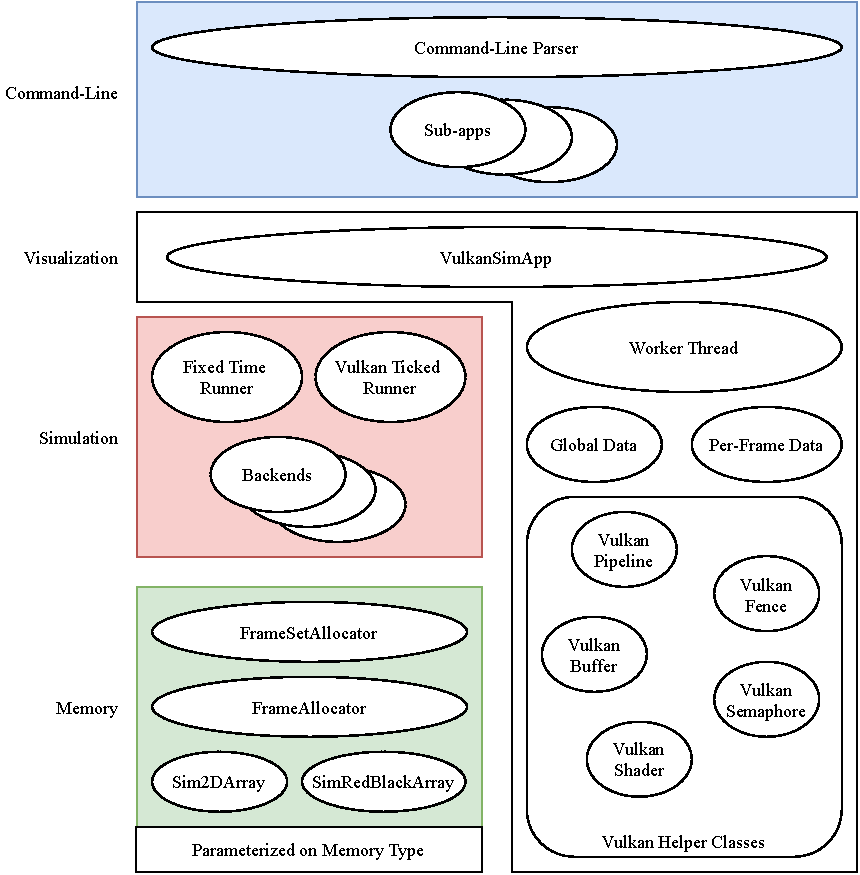
\includegraphics[width=1\linewidth]{Ch42Design/figures/FinalReport_DesignStructure.pdf}}
    \caption{Overall Code Structure}
    \label{fig:designstructure}
\end{figure}
% The overall structure of the project is shown in \cref{fig:designstructure}.
The project structure, shown in \cref{fig:designstructure}, is split into four layers: Command-Line, Visualization, Simulation, and Memory.
Each element broadly represents a C++ class which depends on the classes defined below it.

The Command-Line layer has a Command-Line Parser, which converts the passed-in argument strings to usable representations, and a set of sub-apps.
Each sub-app implements one of the subcommands shown in \cref{sec:DesignSubcommands}.
The figure shows all classes relevant to the \shell{run} subcommand, which shows a visualized simulation.

The Visualization layer contains a high-level \code{VulkanSimApp} class, which initiates all visualization-related code.
Beneath that the Worker Thread handles most Vulkan API calls, and depends on multiple sets of data built with Vulkan helper classes.
This layer uses classes from the Simulation layer, which are reused for the \shell{fixedtime} subcommand to avoid code duplication.

The Simulation layer consists of two main elements: the Runners, and the Backends.
The Runners use different strategies for invoking a Backend - the \code{FixedTimeRunner} runs the simulation flat out until a specific time is reached and outputs the final state, and the \code{VulkanTickedRunner} runs the simulation for a small timesteps while synchronising with other Vulkan elements.
Each Backend implements the same interface, so Runner implementations can be Backend-agnostic.
The \code{FixedTimeRunner} supports all of the defined Backends (see \cref{sec:DesignBackends}), but the \code{VulkanTickedRunner} can only use the Vulkan-compatible CUDA backend.

Finally, the Memory layer exposes APIs for the Backends to allocate simulation memory.
Runners decide how many `frames' to create (see \cref{sec:DesignSimNBuffer}), and use the FrameSetAllocator to create a set of FrameAllocators.
The Backends use each FrameAllocator to allocate a set of buffers, which are then used to store simulation data.
These buffers are represented with Sim2DArray and SimRedBlackArray instances.
The SimRedBlackArray splits a given grid size into two halves, one storing entirely red elements and one storing entirely black elements, and can be configured to store an additional full matrix (helpful for e.g. pressure, where both representations are useful.)

All elements of the Memory layer are parameterized on the type of memory.
This can be CPU memory allocated with \code{malloc} and \code{free}, CUDA Unified Memory (see \cref{sec:Design:Simulation}), or Vulkan on-device memory. 
The memory type affects not just the allocation method, but also the properties it has e.g. CPU memory cannot be accessed from the GPU.
Using parameterized array classes allows these differences to be expressed while keeping a consistent interface.

\section{Simulation \& Memory Layer}
% The simulation component of the program is used in both the headless and real-time modes, so the design needs to be suitable for working with both.

% \subsection{Backends}
To allow easy comparisons between CPU and GPU simulations the program contains multiple simulation backends.
%which can be requested when running a headless simulation\footnote{The realtime visualization currently only supports the CUDA-based backend, violating \cref{req:GPUCapable}.}.
The headless and visualized simulations use a \texttt{--backend} command line option to allow the user to choose the backend from this selection:\label{sec:DesignBackends}
\begin{itemize}
    \item Null, a backend which does no simulation for testing purposes.
    \item CPU Simple, equivalent to pre-optimization ACA code.
    \item CPU Optimized, equivalent to the submission for ACA, bit-equivalent to CPU Simple.
    \item CPU Optimized Adapted, a version of CPU Optimized slightly modified to be closer to the GPU version.
    \item CUDA Backend V1, the only GPU-based backend.
\end{itemize}

The only modification present in the CPU Optimized Adapted backend is the removal of double-precision floating point logic, which is not present on the GPU for speed concerns.
It still isn't identical to the CUDA environment, as CUDA aggressively contracts floating point operations to fused multiply-add while the CPU compiler does not.
The other CPU optimizations are present on the GPU where possible: the residual check between each Poisson phase is still removed, and the red-black data is still separated into separate arrays. 
% However once the GPU introduces residual checking for the iterative solver, or any other major changes to the pipeline, they will be introduced into this backend to ensure a like-for-like comparison.

% Each backend implements a consistent interface (\todoref{UML Figure for interface}), allowing the implementations of the headless and visualized running modes to be backend-agnostic.
% The headless simulation mode can use all of the available backends.
% The visualization only supports the CUDA backend, as it is the only backend which is compatible with Vulkan.
% While the code for the visualized running mode could theoretically use any Vulkan-compatible backend, the CUDA backend is the only Vulkan-compatible backend present in the final program.

\subsection{CUDA Design}\label{sec:Design:Simulation}

The CUDA backend implements each stage of the simulation (\cref{fig:SimStages}) as one or more CUDA Kernels.
Each CUDA Kernel represents a computation for a single grid cell, which is executed by a GPU thread.
The grid is split into small `blocks' of threads, and the threads within each block are executed by a Streaming Multiprocessor (SM) in groups of 32 (a `warp').% in parallel over the entire grid.
% These threads are split into a hierarchy as described in \todocite{https://www.nvidia.com/content/PDF/fermi_white_papers/NVIDIA_Fermi_Compute_Architecture_Whitepaper.pdf}.
% ``A GPU executes one or more kernel grids; a streaming multiprocessor (SM) executes one or more thread blocks; and CUDA cores and other execution units in the SM execute threads.''
The grids and blocks can be specified in 1D, 2D, or 3D depending on the dimensionality of the problem.
Our program uses a 2D grid for most kernels, because each computation reads adjacent data in 2D space.
Reduction kernels treat the 2D grid as a flat 1D array, because there is no need for adjacent data.

The CUDA backend must execute both with Vulkan (when visualized) and without Vulkan (when headless).
This affects the type of memory used in the simulation.
When visualized, crucial data such as velocity and pressure are stored in shared Vulkan-CUDA memory, to allow direct usage from both APIs without copying the data.
In all other cases CUDA Unified Memory is used, which can be paged between the CPU and GPU on-demand without manually mapping it across\cite{Harris2017UnifiedBlog}.
This allowed for granular debugging during development, as GPU kernels could be easily swapped out for known-correct CPU implementations without having to move memory manually.

% \todomark{CUDA Unified memory allows for granular debugging by combining known-correct CPU implementations with GPU kernels} 

\subsection{N-Buffering}\label{sec:DesignSimNBuffer}
When developing the Visualization, it was noted that keeping a separate copy of the simulation output would allow the visualization to run in parallel with the simulation, without the simulation overwriting data currently being visualized.
To allow this, N-buffering was introduced to the simulation backends and to aspects of the visualization.
Multiple `frames' are stored, where each one contains all data used in a simulation tick.
Each simulation tick is assigned to a specific frame chosen by the Runner, and only the data in this frame is written to.
The index of the last-written frame is tracked, and is used as the input for the next simulation tick.
During a simulation of frame \#N, the contents of the other frames is constant and can be read out without any race conditions.

% \subsection{Design Optimizations}
% The residual check after every Poisson phase is still removed, although it was planned to be 

\pagebreak
\section{Visualization Layer}
This section details the code implemented in order to efficiently and effectively visualize simulation results in real time.
This is not related to the \texttt{renderppm} subcommand, which uses CPU code to render a single simulation state as an image.

\subsection{Components}
There are four major components of the visualization which work together to create the final output.
\begin{itemize}
    \item CPU 0 - The Main Thread, which handles the CUDA simulation.
    \item CPU 1 - The Worker Thread, which records and enqueues Vulkan commands.
    \item The GPU, which executes both the CUDA and Vulkan commands.
    \item The Swapchain, which provides render targets that are displayed in the application window.
\end{itemize}
The GPU itself has three phases of execution, performed sequentially for each frame (\cref{tab:gpuexecution}).
Each frame accesses a set of per-frame data, which is reused in a circular buffer.
Each phase for the frame will use this data.
\begin{table}[h]
    \centering
    \begin{tabular}{l|c}
    Name & Abbreviation \\
    \hline
    Simulation & Sim \\
    Visualization Compute (e.g. simulating particles) & VizComp \\
    Visualization Graphics & VizGfx \\
    \end{tabular}
    \caption{GPU Execution Phases, with abbreviations}
    \label{tab:gpuexecution}
\end{table}

A key design goal with the visualization was to maximize GPU utilization.
The CPU work is much less complicated than the GPU work, so the CPU should always be able to keep the GPU fed with new work.
If the CPU failed to do this, the GPU would waste time idling when it could be doing useful work.

\begin{figurepage}
\begin{figure}[p]
    \centering
    \makebox[\textwidth][c]{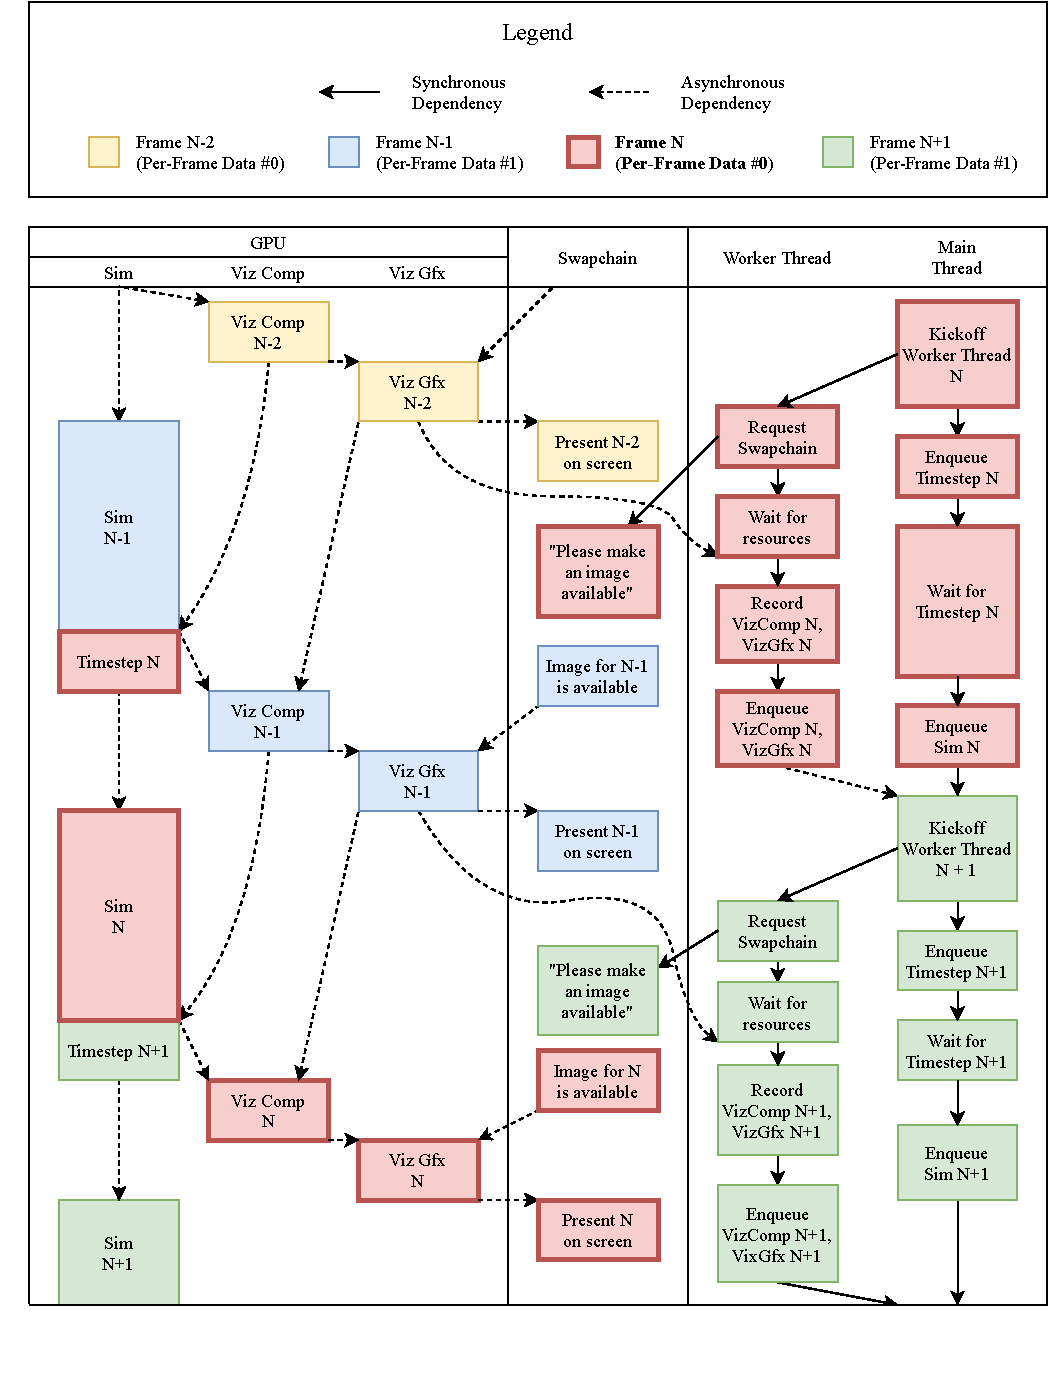
\includegraphics[width=1.1\linewidth]{Ch42Design/figures/FinalReport_Timing.pdf}}
    \caption{Timing Breakdown of four visualization frames, assuming two sets of per-frame data.}
    \label{fig:DesignTiming}
\end{figure}
\end{figurepage}

\subsection{Timing Breakdown}\label{sec:Design:Viz:Timing}

\cref{fig:DesignTiming} shows a breakdown of multiple frames of simulation and visualization, focusing on \textbf{frame \#N} which is highlighted in red.
It includes both synchronous and asynchronous dependencies.
A task with synchronous dependencies starts immediately once all dependencies finish.
A task with asynchronous dependencies can only start once all dependencies are finished, but may not start until later.

The main thread begins by initiating the worker thread before handling the simulation.
Before any CUDA work is enqueued, a semaphore is used to create a dependency on a previous compute job (`Viz Compute $N - 2$'). % Semaphore computeFinishedCanSim.
This compute cycle and the incoming CUDA work will access the same per-frame data\footnote{Viz Gfx jobs don't access the raw simulation buffers, so it doesn't delay the simulation.}, so this dependency prevents the simulation from writing to the data while the compute job reads from it.
For higher efficiency this dependency could be inserted on `Sim $N$' instead, but in practice it would not affect the results.

The VulkanTickedRunner enqueues CUDA work to determine the maximum timestep for the next tick (`Timestep $N$' in the diagram), waiting to get the results back on the CPU, and enqueueing the rest of the simulation based on the calculated timestep (`Sim $N$')\footnote{`Sim' and `Timestep' work are enqueued on the same CUDA stream, so they are implicitly ordered.}.%\todocite{CUDA stream ordered}
If visualization requested a larger timestep than the calculated maximum, the process would be repeated until the total requested timestep had elapsed.
Once `Sim $N$' is finished, it signals a semaphore to allow `Viz Comp $N$' to continue the frame. % Semaphore simFinishedCanCompute

The worker thread asks the swapchain for an image using the \texttt{vkAcquireNextImageKHR} function.
This returns an index which will eventually become available, and a semaphore which will be signalled once this happens.
Before `Viz Gfx $N$' can render to this image, it has to wait for this semaphore to signal it is ready. % Semaphore imageAcquiredCanRender
The thread then waits for frame $N-2$ to finish using the Vulkan resources in Resource Set 0, before it uses them to record `Viz Comp $N$' and `Viz Gfx $N$'. % Fence frameCmdBuffersInUse
The Viz jobs have some semaphores to guarantee ordering:
`Viz Gfx $N$' must start after `Viz Comp $N$' finishes, which must start after `Sim $N$' finishes. % Semaphore simFinishedCanCompute, computeFinishedCanRender
`Viz Comp $N$' also has to wait for `Viz Gfx $N - 1$' to finish to avoid race conditions - all `Viz Comp' and `Viz Gfx' jobs share global memory instead of per-frame memory to avoid data copying. % Semaphore renderFinishedNextFrameCanCompute
Once `Viz Gfx $N$' finishes, it signals a semaphore to tell the swapchain/OS to present the newly rendered frame to the screen.
The worker thread records and enqueues the above work for the GPU.
Once the worker thread has finished it signals the main thread, and once the main thread finishes enqeueing `Sim $N$' the process restarts.

It's worth noting that based on these dependencies some GPU work could theoretically run in parallel, such as `Viz Comp $N$' and `Timestep $N-1$'.
Unfortunately in practice this doesn't happen.
Running parallel compute workloads was introduced in the Ampere GPU generation \cite{nvidiaAmpereWhitepaper}, such as the RTX~3000 series, and is not supported on the researcher's GTX~1080.
This also affects the work breakdown, preventing smaller pieces of work (such as computations for separate visualization layers) from running in parallel.
In the future this could be mitigated by using an Ampere-level GPU, or by running the simulation and visualization on separate GPUs.

\subsubsection{Synchronization}
In order to implement an unlocked framerate without running the simulation faster than real-time, the time between frame `starts'\footnote{i.e. kicking off the worker thread} is measured to determine how long an average simulation frame takes. 
% The desired `simulations-per-second' is set by the user, and 
The program predicts how long a simulation frame \emph{would} take, and combines that with the requested simulation rate\footnote{e.g. 120 simulation ticks per second} to predict if the next frame should be a simulation frame.

When running with an unlocked simulation rate, the average time per simulation frame is chosen as the timestep for the next simulation tick.
This is capped with sensible minimum/maximum limits to avoid instability from performance outliers.

\subsection{Visualization Work Breakdown}\label{sec:Design:Viz:Breakdown}
As specified in the Requirements (\cref{sec:Requirements}) the selected visualization layers are the Background, Quantity-by-Scalar, Quantity-by-Vector, and Particle Simulation.
The Background and Quantity-by-Scalar layers are visualized at the same time for simplicity.
Accounting for this, the breakdown of required work for each layer is shown in \cref{fig:VizBreakdown}.

\begin{figure}
    \centering
    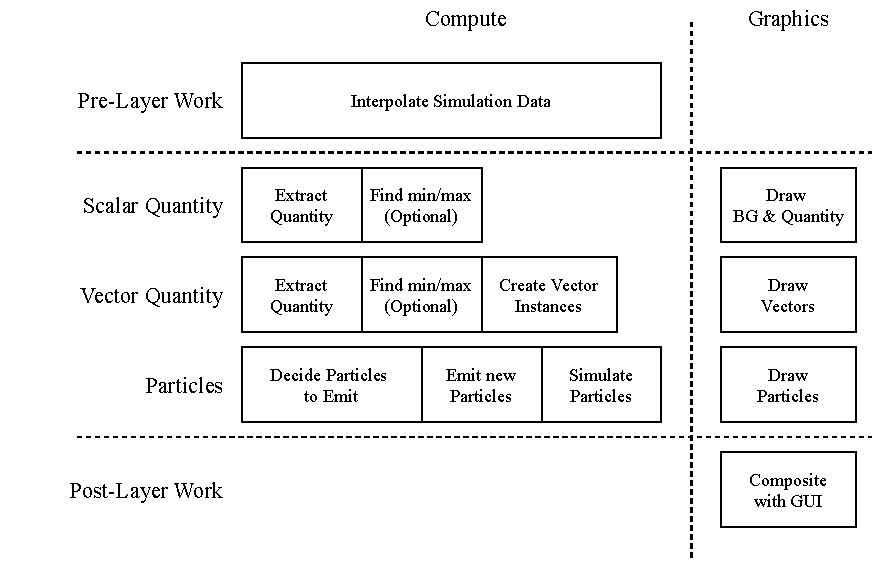
\includegraphics[width=\linewidth]{Ch42Design/figures/FinalReport_VizWork.pdf}
    \caption{Visualization Work Breakdown}
    \label{fig:VizBreakdown}
\end{figure}

The Compute sections are implemented using Vulkan Compute Shaders\cite{TheKhronosGroupVulkanSpec}, which are nearly equivalent to CUDA Kernels and are invoked similarly.
The Graphics sections are implemented using Vertex and Fragment Shaders, where the Vertex Shader determines the onscreen positions of the vertices that make up a model, and the Fragment Shader determines the color of the onscreen pixels between those vertices.

\subsubsection{Data Interpolation}
The simulation stores data on a staggered grid (\cref{fig:staggered_grid}), but this is not amenable for some visualization tasks.
The first step of the visualization is to move the exposed simulation data into a 2x resolution texture, applying interpolation where necessary, allowing the GPU to sample the exposed data at arbitrary points using the texture filtering hardware.
This applies trilinear interpolation, as required for the particle simulation.

\subsubsection{Auto-ranging}
Both Quantity-by-Scalar and Quantity-by-Vector have an optional auto-range mode, where the minimum and maximum values for the quantity are calculated and used instead of the user-defined quantity scale.
This requires a GPU reduction, which is implemented in Vulkan just like it is in CUDA, using the second kernel of \cite{CUDAParallelReduction}.
In order to easily render the data in both cases the selected quantity is extracted to two buffers using a specialized compute shader.
The first buffer includes the quantity with a `fluidmask' which shows if the selected pixel is a fluid or obstacle, and is used for the rendering.
The second buffer has a min/max property for each element, and is used as the input to the reduction.

\subsubsection{Indirect Instanced Rendering}
For Quantity-by-Vector and the Particle Simulation, the final outputs are rendered using Instanced Rendering.%\todocite{Instanced Rnedering}
The same model is rendered $N$ times, and the Vertex Shader gets an `instance index' $0 \le i < N$.
This index is used to look-up the instance's position/orientation in a separate buffer.
This method is much faster than rendering each instance separately, as it requires fewer draw calls on the CPU.
\begin{figure}
    \centering
    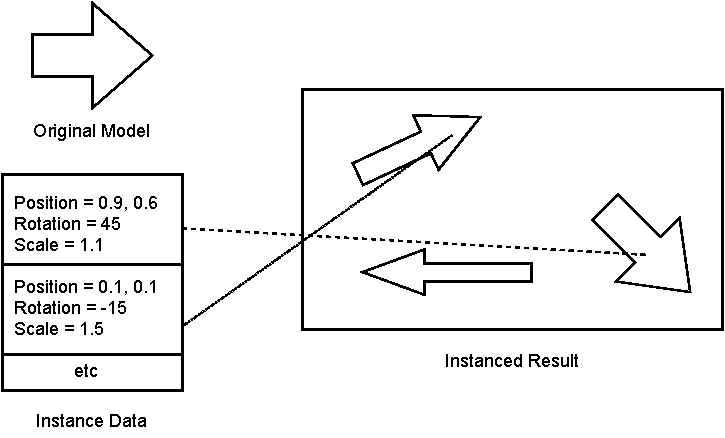
\includegraphics{Ch42Design/figures/FinalReport_InstancedRendering.pdf}
    \caption{Instanced Rendering Demonstration}
    \label{fig:InstancedRendering}
\end{figure}

When recording the command buffer on the CPU, the number of instances for both layers is not yet known.
For Quantity-by-Vector the number of vectors is dependent on the simulation output, because vectors cannot be placed on obstacles.
Some Particles may be killed by the previous round of simulation, so they cannot be predicted either.
To mitigate this, Indirect invocations are used for the vector/particle rendering and the particle simulation.
Instead of specifying the instance count at record time, a reference to a GPU buffer is used.
This GPU buffer contains the required parameters for the instanced rendering/compute dispatch, and can be atomically written by the GPU in a separate compute shader.

Creating new vectors/particle instances is done safely on the GPU using growable lists and atomic variables.
Each growable list consists of an array of values with a maximum length, and a `current size' variable.
When a value is added, the `current size' variable is incremented atomically, and the pre-increment value is then used to index the array and write the new instance parameter.
When a value is removed, the `current size' variable is decremented atomically, and the post-increment value can be used to see the deleted value.
Within a compute shader invocation, a list can only be growable or shrinkable but cannot be both.
Despite this limitation the lists are suitable to implement the technique from \cite{WickedEngineParticles}.

\subsubsection{Final Composite}
As a final step the visualization output is rendered with the other GUI elements.
This step is controlled by the Dear ImGUI library, not my own code (see \cref{sec:LibrarySelection}).
An example of the visualization GUI is shown in \cref{fig:viz_gui}.

\begin{figure}[b]
    \centering
    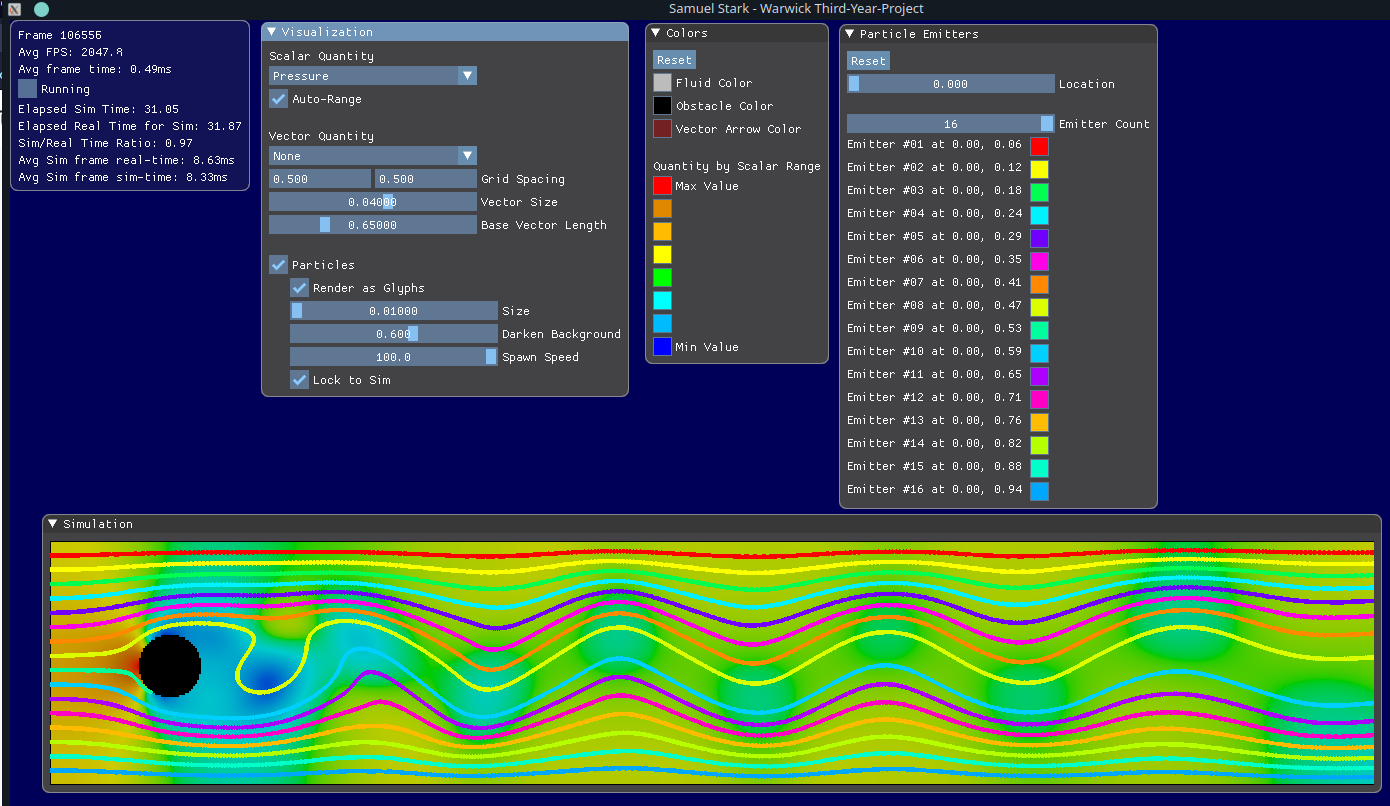
\includegraphics[width=\linewidth]{Ch42Design/figures/dan.png}
    \caption{Example of the Visualization GUI}
    \label{fig:viz_gui}
\end{figure}


\section{Command-Line Layer \& Program Usage}
% \todomark{intro para?}

% \subsection{Command-Line Interface}
The compiled binary uses a command-line interface to configure and run one of many subcommands available.
These subcommands are:\label{sec:DesignSubcommands}
\begin{itemize}
    \item \texttt{makeinput}, which generates simulation input files, fulfilling \cref{req:GenerateState}.
    \item \texttt{fixedtime}, which runs a headless simulation for a fixed time, fulfilling \cref{req:HeadlessSim}.
    \item \texttt{compare}, which compares two simulation states for equality (see \cref{sec:Comparisons}), fulfilling \cref{req:Compare}.
    \item \texttt{renderppm}, which visualizes a static simulation state using the techniques from \cref{sec:Research:Viz:ACA}.
    % \item \texttt{convert2newbinary}, for converting ACA simulation state files to a potential new format (see \cref{sec:FileFormat}). Currently a no-op.
    \item \texttt{run}, which starts a real-time visualized simulation, fulfilling \cref{req:VizSim}.
\end{itemize}
Splitting the program into subcommands was inspired by Git\cite{tool:Git}, and avoids creating separate binaries for each operation.
Each subcommand can be configured with command-line options conforming to POSIX standard\cite{IEEE2018UtilityConventions}.
Examples of using the program are in \cref{fig:BashExampleUsage}.
\begin{figure}[ht]
    \centering
    \begin{lstlisting}[language=bash]
# Create an input file based on simple_layout with a size of 1x2 metres
./sim_cuda makeinput ./simple_layout.png 1 2 ./initial.bin

# Run it in headless mode for 10 seconds
./sim_cuda fixedtime --backend=cuda ./fluid.json ./initial.bin 10 \
                        -o ./output_after_10.bin

# Compare it to the expected output
./sim_cuda compare ./output_after_10.bin ./expected_after_10.bin

# Render it out to an image
./sim_cuda renderppm ./output_after_10.bin zeta ./output_after_10.ppm

# Try visualizing it in real-time
./sim_cuda run --backend=cuda ./fluid.json ./initial.bin
\end{lstlisting}
    \caption{Example usage of the simulation program}
    \label{fig:BashExampleUsage}
\end{figure}

\subsection{Generating Inputs}
The \texttt{makeinput} subcommand allows input simulation states to be generated from image files.
Each pixel of the input image represents a cell of the grid, including padding cells\footnote{This can allow the padding cells to be fluids rather than boundaries, which is incorrect. In the future this will be changed to add padding cells once the image is parsed.}, where non-black pixels are denoted as boundary cells and are fluid cells otherwise.
The example in \cref{fig:ExampleMakeinput} shows an example file which creates a rectangular obstacle, and the visualization of the generated state.
\begin{figure}[ht]
    \centering

    \subcaptionbox{Base Image%
    }[\linewidth]{
\includegraphics[]{Ch42Design/figures/simple_layout.png}
    }
    
    \subcaptionbox{Simulation%
    }[\linewidth]{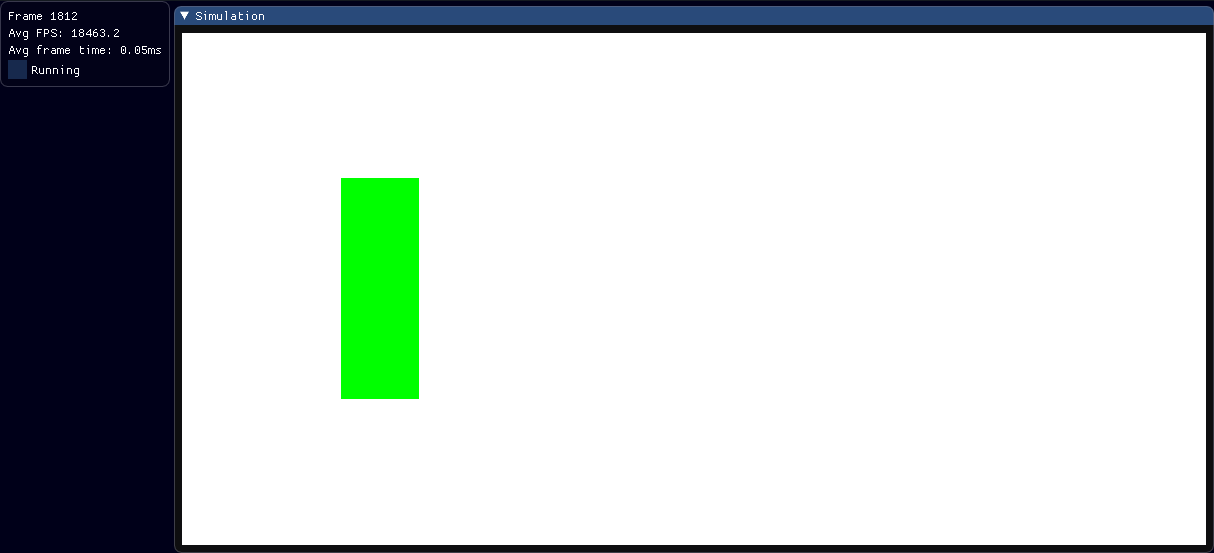
\includegraphics[width=0.5\linewidth]{Ch42Design/figures/example_sim_of_simple_layout.png}
    }
    
    \caption{Example conversion of an image to a simulation state}
    \label{fig:ExampleMakeinput}
\end{figure}

Velocities and pressure in every cell are interpolated horizontally - \SI{1}{m/s} east at the left edge, \SI{0}{m/s} at the right.
This alleviates simulation instability near obstacle edges, an advantage over having a constant initial velocity across the field.
% For velocities, this is \SI{1}{m/s} east, equal to the default flow of incoming fluid, which may cause issues with correctness.
One such instability would be a situation where fluid is occluded from the input direction by an obstacle, but moves east anyway with no reason to do so.
%it would not be correct for that fluid to move) 
% This will likely be changed to zero out initial velocity, requiring some simulation to take place before the fluid begins to move.

The exact initial value of pressure is inconsequential as the simulation only cares about the difference between cells.
The pressure is set to 0 at all points, representing a constant pressure across the simulation grid.
This is inconsistent with the nonzero velocities mentioned above, but applying variable pressure made the system more unstable.

\subsection{File Formats}\label{sec:FileFormat}
To fulfil \cref{req:StoreState} two file formats have been defined to store simulation data and parameters.

\subsubsection{Fluid Parameters}
Parameters that are characteristic of a particular fluid or simulation type are stored in a ``Fluid Parameters'' file.
This includes the Reynolds number, the timestep safety factor, and the maximum iteration count for the Poisson solver.
They are stored in a JSON format to be human-readable, are reusable for different simulation states, and can be easily edited by the end user.
An example is shown in \cref{fig:FluidParamsExample}.

\begin{figure}[ht]
% \begin{wrapfigure}{r}{0.5\textwidth}
    \centering
    %\begin{minted}{json}
    \begin{lstlisting}[language=JSON]
{
    "Re": 150.0,
    "initial_velocity_x": 1.0,
    "initial_velocity_y": 0.0,
    "timestep_divisor": 60,
    "max_timestep_divisor": 480,
    "timestep_safety": 0.5,
    "gamma": 0.9,
    "poisson_max_iterations": 100,
    "poisson_error_threshold": 0.001,
    "poisson_omega": 1.7
}
\end{lstlisting}
% \end{minted}
    \caption{An example Fluid Parameters file.}
    \label{fig:FluidParamsExample}
% \end{wrapfigure}
\end{figure}

\subsubsection{Simulation State}
Data unique to an individual state such as simulation resolution, physical size, and velocity fields are stored in a binary format reused from the original simulation.
As the data is much more sensitive to individual modifications\footnote{i.e. changing a single value in the velocity field can introduce discontinuities}, it makes more sense to store this data in a binary format where it cannot be easily modified by a user.
Additionally, the binary format is much smaller than any text-based format, which helps as the volume of data stored is much larger than that stored in the fluid parameters.

The header consists of a pair of unsigned 32-bit integers specifying the resolution of the simulation, and a pair of 32-bit floating-point numbers specifying the physical dimensions of the simulation.
From there, four sets of data for each column are stored, including the boundary padding squares:
\begin{enumerate}
    \item Horizontal Velocity $u$ (\code{float32})
    \item Vertical Velocity $v$ (\code{float32})
    \item Pressure $p$ (\code{float32})
    \item Cell Flags, defining which adjacent squares are boundaries (\code{uint8})
\end{enumerate}
This structure is somewhat unintuitive and error-prone, an example being the Cell Flags which may end up being inconsistent between adjacent cells, but it has been kept for the sake of compatibility with the original simulation.


\subsection{Comparison Heuristics}\label{sec:Comparisons}
In the \shell{compare} subcommand heuristics are used to judge if one simulation is accurate and precise with respect to the other.
This does not quite fulfil \cref{req:CompareBinary}, as there are two results and two heuristics used instead of just one, but it is useful for comparisons regardless so was not changed.

This assumes one of the supplied states is a known-valid simulation state, and the other is not.
The velocity and pressure values $u, v, p$ of the two simulation states are compared separately.
% The simulation states must be of the same resolution, and should use the same boundary squares (although this is not checked).
The simulation states must be of the same size and use the same obstacle squares.

The comparison is performed by calculating the mean and standard deviation of the square error between the datasets.
These are then compared to tolerance values to produce two binary outputs: ACCURATE if the mean is below tolerance, and PRECISE if the standard deviation is below tolerance.
Examples are shown in \cref{fig:example_comparisons}.

The tolerance for the mean was derived from an expected error magnitude of $\pm 10^{-7}$, which was squared to produce $10^{-14}$.
It is assumed that the standard deviation should always be smaller than the mean, so the tolerance for standard deviation is also $10^{-14}$.
% \todopending{More examination of this? Square error always >0 => if std.dev > mean then distribution cannot be normal? Prob wait for full report}

\begin{figure}[ht]
    \centering
    \begin{center}
    \lstset{language=bash,
    numbers=none,
    keywordstyle=[2]\color{red},
    keywords=[2]{INACCURATE,IMPRECISE},
    keywordstyle=[3]\color{green},
    keywords=[3]{ACCURATE,PRECISE}
    }
    % \lstset{language=bash,
    % linewidth=0.5\linewidth
    % % keywordstyle=[2]\color{red},
    % % keywords=[2]{INACCURATE,IMPRECISE},
    % % keywordstyle=[3]\color{green},
    % % keywords=[3]{ACCURATE,PRECISE}
    % }
    % \subcaptionbox{Comparison of equal states}[0.5\linewidth]{\begin{frame}[fragile]\end{frame}}
    %[xleftmargin=-0.2\textwidth]
\begin{subfigure}{0.4\textwidth}\begin{lstlisting}
Velocity X:
    Sq. Error Mean:     0     ACCURATE
    Sq. Error Std. Dev: 0     PRECISE
Velocity Y:
    Sq. Error Mean:     0     ACCURATE
    Sq. Error Std. Dev: 0     PRECISE
Pressure:
    Sq. Error Mean:     0     ACCURATE
    Sq. Error Std. Dev: 0     PRECISE\end{lstlisting}%
    \caption{Comparison of Equal States}%
\end{subfigure}%
\hspace{0.02\textwidth}
\begin{subfigure}{0.5\textwidth}\begin{lstlisting}[]
Velocity X:
    Sq. Error Mean:     0.0233842     INACCURATE
    Sq. Error Std. Dev: 0.0996487     IMPRECISE
Velocity Y:
    Sq. Error Mean:     0.00566354    INACCURATE
    Sq. Error Std. Dev: 0.0139529     IMPRECISE
Pressure:
    Sq. Error Mean:     0.0214799     INACCURATE
    Sq. Error Std. Dev: 0.0511252     IMPRECISE\end{lstlisting}%
\caption{Comparison of Unequal States}%
\end{subfigure}
\end{center}
% Velocity X:
%         Sq. Error Mean:                   0     ACCURATE
%         Sq. Error Std. Dev:               0     PRECISE
% Velocity Y:
%         Sq. Error Mean:                   0     ACCURATE
%         Sq. Error Std. Dev:               0     PRECISE
% Pressure:
%         Sq. Error Mean:                   0     ACCURATE
%         Sq. Error Std. Dev:               0     PRECISE
    
%     \subcaptionbox{Comparison of unequal states%
%     }[0.5\linewidth]{\begin{lstlisting}
% Velocity X:
%         Sq. Error Mean:           0.0233842     INACCURATE
%         Sq. Error Std. Dev:       0.0996487     IMPRECISE
% Velocity Y:
%         Sq. Error Mean:          0.00566354     INACCURATE
%         Sq. Error Std. Dev:       0.0139529     IMPRECISE
% Pressure:
%         Sq. Error Mean:           0.0214799     INACCURATE
%         Sq. Error Std. Dev:       0.0511252     IMPRECISE
% \end{lstlisting}}
    
    \caption{Examples outputs from the comparison tool.}
    \label{fig:example_comparisons}
\end{figure}

% % \todomark{UI}

